% Propósito: distinguir reflexión, absorción y transmisión como destinos
% simultáneos de la energía incidente.
% Origen: balance ideal R + alpha + tau = 1. Las flechas no codifican valores.
% Accesibilidad: una onda incide sobre una partición; una fracción regresa,
% otra se disipa en la partición y otra pasa al segundo recinto.
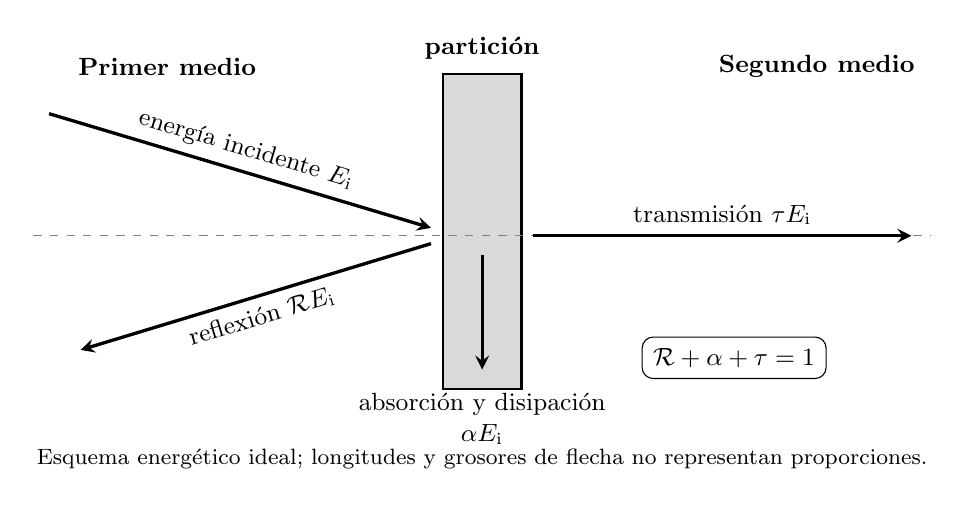
\begin{tikzpicture}[
    x=1cm,
    y=1cm,
    >=stealth,
    font=\small,
    flujo/.style={very thick,->},
    guia/.style={gray,dashed}
]
    \node[font=\small\bfseries] at (2.25,4.75) {Primer medio};
    \node[font=\small\bfseries] at (10.50,4.75) {Segundo medio};

    \path[fill=black!15] (5.75,0.65) rectangle (6.75,4.65);
    \draw[thick] (5.75,0.65) rectangle (6.75,4.65);
    \node[font=\small\bfseries,anchor=south] at (6.25,4.72) {partición};
    \draw[guia] (0.55,2.60) -- (11.95,2.60);

    \draw[flujo] (0.75,4.15) -- (5.60,2.70)
        node[midway,above,sloped] {energía incidente \(E_\mathrm{i}\)};
    \draw[flujo] (5.60,2.50) -- (1.15,1.15)
        node[midway,below,sloped] {reflexión \(\mathcal{R}E_\mathrm{i}\)};
    \draw[flujo] (6.90,2.60) -- (11.70,2.60)
        node[midway,above] {transmisión \(\tau E_\mathrm{i}\)};
    \draw[flujo] (6.25,2.35) -- (6.25,0.90);
    \node[align=center,anchor=north] at (6.25,0.72)
        {absorción y disipación\\\(\alpha E_\mathrm{i}\)};

    \node[draw,rounded corners,fill=white,inner sep=4pt]
        at (9.45,1.05) {\(\mathcal{R}+\alpha+\tau=1\)};
    \node[font=\footnotesize,anchor=north] at (6.25,0.02)
        {Esquema energético ideal; longitudes y grosores de flecha no representan proporciones.};
\end{tikzpicture}
